\documentclass{myart}
\usepackage{caption}
\usepackage{enumitem}
\usepackage{tikz}

\allowdisplaybreaks

\newcommand{\eq}[1]{(\ref{eq:#1})}
\newcommand{\Figure}[1]{Figure \ref{fig:#1}}

\begin{document}

\titlepage
{The Existence-Uniqueness Theorem for First-Order Differential
  Equations}
{picard-lindelof-theorem}
{This document is a proof of the existence-uniqueness theorem for
  first-order differential equations, also known as the
  Picard-Lindel\"of or Cauchy-Lipschitz theorem. It was written with
  special attention to both rigor and clarity. The proof is primarily
  based on the one given in the textbook I used in my Differential
  Equations class (\textit{Differential Equations and Their
    Applications} by Martin Braun, fourth edition).}

\section{Goal}

Let $f$ be a function of two variables and let $t_0$ and $y_0$ be real
numbers. This defines an initial-value problem:
\begin{align} \label{eq:ivp}
\begin{split}
y'(t) &= f(t, y(t)) \\
y(t_0) &= y_0.
\end{split}
\end{align}
Our goal is to prove that under certain conditions, there is exactly
one solution $y$ to this differential equation. That is, we would like
to prove both the \emph{existence} and \emph{uniqueness} of solutions
to the equation.

\section{Initial Steps}

We will start our proof by transforming the differential equation
\eq{ivp} into a more convenient form. This is done by integrating both
sides from $t_0$ to $t$:
\begin{equation*}
\int_{t_0}^t y'(\tau) \,d\tau = \int_{t_0}^t f(\tau, y(\tau)) \,d\tau.
\end{equation*}
Here, to avoid ambiguity, we are using the variable $\tau$ as our
variable of integration instead of $t$. The above equation reduces to
\begin{equation*}
y(t) - y_0 = \int_{t_0}^t f(\tau, y(\tau)) \,d\tau,
\end{equation*}
since $y(t_0) = y_0$, and solving for $y(t)$ gives the equation
\begin{equation} \label{eq:machine}
y(t) = y_0 + \int_{t_0}^t f(\tau, y(\tau)) \,d\tau.
\end{equation}
By this reasoning, any function satisfying \eq{ivp} must also satisfy
equation \eq{machine}. However, the converse statement requires a
little more work. Suppose that a function $y$ satisfies equation
\eq{machine}. Then it follows immediately that $y(t_0) = y_0$, because
\begin{equation*}
y(t_0) = y_0 + \int_{t_0}^{t_0} f(\tau, y(\tau)) \,d\tau = y_0.
\end{equation*}

Now, the fundamental theorem of calculus tells us that if a function
$f$ is continuous, then $\int_a^b f(x)\,dx$ is differentiable with
respect to $b$, and
\begin{equation*}
\frac{d}{db} \int_a^b f(x) \,dx = f(b).
\end{equation*}
Hence, if we assume that if both $f$ and $y$ are continuous, then
$f(\tau, y(\tau))$ is a continuous function of $\tau$ and we have
\begin{equation*}
y'(t) = \frac{d}{dt} \int_{t_0}^t f(\tau, y(\tau)) \,d\tau = f(t, y(t)).
\end{equation*}
Therefore, if $y$ is a continuous function satisfying \eq{machine} and
$f$ is continuous, then $y$ is a solution of the original differential
equation \eq{ivp}.

\section{Outline}

Our proof will consist of the following major steps:
\begin{enumerate}[label=(\alph*)]
\item Construct a sequence of functions $\{y_0(t), y_1(t), \ldots\}$,
  called Picard iterates, which approximate a solution to the equation
  \eq{machine}.
\item Show that the sequence of functions converges and define $y(t) =
  \lim_{n \to \infty} y_n(t)$.
\item Show that the function $y(t)$ satisfies equation \eq{machine}.
\item Show that the function $y(t)$ is continuous.
\item Show that there can only be one solution to the equation
  \eq{machine}.
\end{enumerate}
Having completed these tasks, our reasoning above will imply that the
function $y(t)$ is the unique solution to \eq{ivp}.

\section{Construction of the Picard iterates}

As our first approximation to a solution to the differential equation
\eq{ivp}, we will choose the simplest possible function that satisfies
the condition $y(t_0) = y_0$; that is,
\begin{equation*}
y_0(t) = y_0.
\end{equation*}
Our procedure for generating better approximations is motivated by the
relation \eq{machine} which is satisfied by any solution $y$ to
\eq{ivp}, reprinted here:
\begin{equation*}
y(t) = y_0 + \int_{t_0}^t f(\tau, y(\tau)) \,d\tau.
\end{equation*}
In particular, we will define
\begin{equation} \label{eq:picard}
y_n(t) = y_0 + \int_{t_0}^t f(\tau, y_{n-1}(\tau)) \,d\tau
\end{equation}
for every $n \geq 1$. Observe that we have $y_n(t_0) = y_0$ for every
$n \geq 0$, so every Picard iterate obeys the initial condition.

As a concrete example of this iteration process, consider the
differential equation
\begin{align*}
y'(t) &= y(t) \\
y(0) &= 1,
\end{align*}
whose unique solution is $y(t) = e^t$. For this equation, we have
$f(t, y) = y$, $t_0 = 0$, and $y_0 = 1$. This transforms the
recurrence relation \eq{picard} to
\begin{equation*}
y_n(t) = 1 + \int_0^t y_{n-1}(\tau) \,d\tau;
\end{equation*}
therefore,
\begin{align*}
y_0(t) &= 1 \\
y_1(t) &= 1 + \int_0^t \,d\tau = 1 + t \\
y_2(t) &= 1 + \int_0^t 1 + \tau \,d\tau = 1 + t + \frac{t^2}{2} \\
&\mathrel{\makebox[\widthof{=}]{\vdots}} \\
y_n(t) &= 1 + t + \frac{t^2}{2} + \cdots + \frac{t^n}{n!}.
\end{align*}
The astute reader will recognize $y_n(t)$ as the $n$th partial sum of
the Maclaurin series for $e^t$. It follows easily, then, that the
sequence $\{y_0(t), y_1(t), \ldots\}$ converges and that the limiting
function $y(t) = \lim_{n \to \infty} y_n(t) = e^t$ is continuous and
satisfies \eq{machine}. We now show that this conclusion is true in
general under suitable assumptions.

\section{Bounding the Picard iterates}

In general, even if the differential equation \eq{ivp} has a unique
solution, the solution may only be valid on a specified
interval---typically because $f(t, y(t))$ is not defined for one or
more values of $t$. Therefore, we will have to restrict our reasoning
to a limited interval containing $t_0$. However, it is difficult to
reason about the largest possible interval---that is, the largest
interval over which the differential equation has a solution. Instead,
we will pick a smaller interval in such a way that the behavior of the
Picard iterates is easy to analyze over the interval.

To construct this interval, we will start by picking two arbitrary
positive real numbers $a$ and $b$. These numbers define a rectangle in
the $t$-$y$ plane that has vertices at $(t_0, y_0 - b)$, $(t_0, y_0 +
b)$, $(t_0 + a, y_0 - b)$, and $(t_0 + a, y_0 + b)$. This rectangle is
illustrated in \Figure{rectangle}.

\begin{figure}[htb!]
\begin{tikzpicture}[declare function={ f(\x) = 1.5*exp(-\x/5); }]
\draw [->] (-2.8, -1) -- (8.25, -1) node [right] {$t$};
\draw [->] (-2.5, -1.3) -- (-2.5, 4) node [above] {$y$};
\draw (0, 0) rectangle (5, 3);
\foreach \x/\y/\side/\xcoord/\ycoord in {
	0/1.5/above right/t_0/y_0,
	0/0/below left/t_0/y_0 - b,
	0/3/above left/t_0/y_0 + b,
	5/0/below right/t_0 + a/y_0 - b,
	5/3/above right/t_0 + a/y_b + b
	} {
	\fill (\x, \y) circle (1.5pt) node [\side] {$(\xcoord, \ycoord)$};
}
\draw [dashed] (-2.5, 0) node [left] {$y_0 - b$} -- (0, 0);
\draw [dashed] (-2.5, 1.5) node [left] {$y_0$} -- (0, 1.5);
\draw [dashed] (-2.5, 3) node [left] {$y_0 + b$} -- (0, 3);
\draw [dashed] (0, -1) node [below=1pt] {$t_0$} -- (0, 0);
\draw [dashed] (5, -1) node [below=1pt] {$t_0 + a$} -- (5, 0);
\draw [<->, domain=-2:6] plot(\x, {f(\x)});
\draw [help lines] (2, {f(2)}) -- +(0.7, 0.5)
  node [above right, black] {$y = y(t)$};
\end{tikzpicture}
\caption{}
\label{fig:rectangle}
\end{figure}

Let $R$ denote the rectangle and its interior, i.e. the set of all
points $(t, y)$ such that $t_0 \leq t \leq t_0 + a$ and $y_0 - b \leq
y \leq y_0 + b$. Since we are assuming that $f$ is continuous, it
follows that $|f|$ is continuous and has a maximum value on $R$. We
let $M$ denote this maximum value, i.e.
\begin{equation*}
M = \max_{(t, y) \in R} |f(t, y)|.
\end{equation*}
Next, we consider the lines through the point $(t_0, y_0)$ that have
slope $M$ and $-M$, respectively. These lines have equations $y = y_0
\pm M(t - t_0)$, and are shown in \Figure{lines}.

\begin{figure}[htb!]
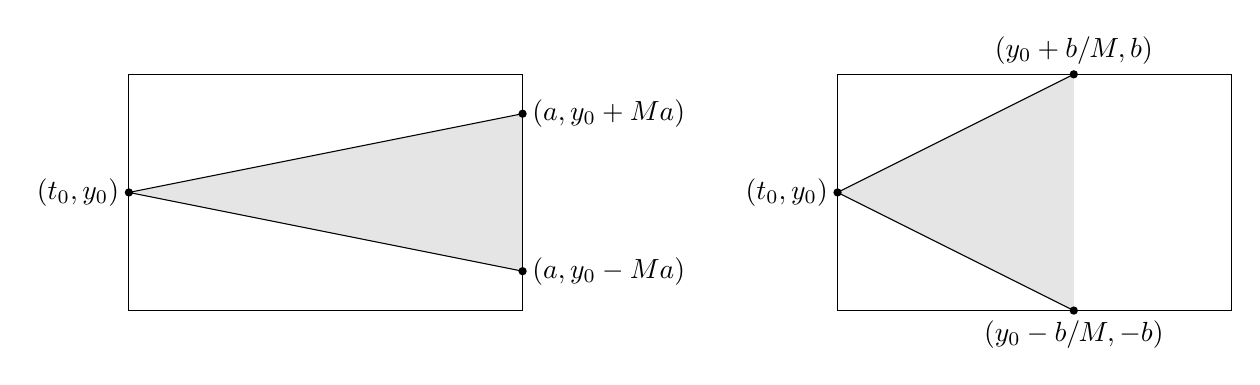
\begin{tikzpicture}
\fill [black!10] (0, 1.5) -- (5, 2.5) -- (5, 0.5) -- cycle;
\draw (0, 0) rectangle (5, 3);
\draw (0, 1.5) -- (5, 2.5);
\draw (0, 1.5) -- (5, 0.5);
\foreach \x/\y/\side/\xcoord/\ycoord in {
	0/1.5/left/t_0/y_0,
	5/2.5/right/a/y_0 + Ma,
	5/0.5/right/a/y_0 - Ma
	} {
	\fill (\x, \y) circle (1.5pt) node [\side] {$(\xcoord, \ycoord)$};
}

\fill [black!10] (9, 1.5) -- (12, 3) -- (12, 0) -- cycle;
\draw (9, 0) rectangle (14, 3);
\draw (9, 1.5) -- (12, 3);
\draw (9, 1.5) -- (12, 0);
\foreach \x/\y/\side/\xcoord/\ycoord in {
	9/1.5/left/t_0/y_0,
	12/3/above/{y_0 + b/M}/b,
	12/0/below/{y_0 - b/M}/-b
	} {
	\fill (\x, \y) circle (1.5pt) node [\side] {$(\xcoord, \ycoord)$};
}
\end{tikzpicture}
\caption{}
\label{fig:lines}
\end{figure}

From the figure, it is easy to see that depending on the value of $M$,
the lines will leave the rectangle at either $t = a$ or $t = b/M$,
whichever is smaller. We will denote this $t$-value by $\alpha$, i.e.
\begin{equation*}
\alpha = \min\left(a, \frac{b}{M}\right).
\end{equation*}
We will now prove that for $t_0 \leq t \leq t_0 + \alpha$, every
Picard iterate lies between the two lines. That is, until the lines
leave the rectangle $R$, every $y_n(t)$ lies within the shaded regions
in \Figure{lines}. We can reformulate this hypothesis as follows:
\begin{align*}
y_0 - M(t - t_0) &\leq y_n(t) \leq y_0 + M(t - t_0) \\
-M(t - t_0) &\leq y_n(t) - y_0 \leq M(t - t_0) \\
|y_n(t) - y_0| &\leq M(t - t_0).
\end{align*}
Because $M \geq 0$ and $t \geq t_0$, we need no absolute value bars on
the right-hand side.

To prove the hypothesis, we use induction on $n$. The case of $n = 0$
follows immediately, as
\begin{equation*}
|y_0(t) - y_0| = |y_0 - y_0| = 0 \leq M(t - t_0).
\end{equation*}
For the inductive case, we assume---for some $n \geq 0$---that
$|y_n(t) - y_0| \leq M(t - t_0)$ for $t_0 \leq t \leq \alpha$ and seek
to prove that $|y_{n+1}(t) - y_0| \leq M(t - t_0)$ on the same
interval. We now use the definition \eq{picard} of the Picard
iterates, reprinted here:
\begin{equation*}
y_{n+1}(t) = y_0 + \int_{t_0}^t f(\tau, y_n(\tau)) \,d\tau.
\end{equation*}
In particular, we note that
\begin{equation*}
|y_{n+1}(t) - y_0| = \left|\int_{t_0}^t f(\tau, y_n(\tau)) \,d\tau\right|.
\end{equation*}
Next, we use the following two elementary properties of definite
integrals:
\begin{align*}
      \left|\int_a^b f(x) \,dx\right|
&\leq \int_a^b |f(x)| \,dx \\
      \int_a^b f(x)|g(x)| \,dx
&\leq \left(\max_{a \leq x \leq b} f(x)\right)\int_a^b |g(x)| \,dx.
\end{align*}
Note that we have $t_0 \leq \tau \leq t \leq t_0 + \alpha$.
Consequently, it follows from the inductive hypothesis that
$y_n(\tau)$ lies between the lines and hence within $R$ on this
interval. Thus, $(\tau, y_n(\tau))$ lies within $R$ for all $\tau$
from $t_0$ to $t$, and $|f(\tau, y_n(\tau))| \leq M$ over this
interval. From these properties, we have:
\begin{align*}
      \left|\int_{t_0}^t f(\tau, y_n(\tau)) \,d\tau\right|
&\leq \int_{t_0}^t |f(\tau, y_n(\tau))| \,d\tau \\
&\leq M(t - t_0).
\end{align*}
We have therefore shown that $|y_{n+1}(t) - y_0| \leq M(t - t_0)$,
which completes the proof that $|y_n(t) - y_0| \leq M(t - t_0)$ for
every $n \geq 0$.

\section{Proof that the Picard iterates converge}

Now that we have obtained a bound on the size of $y_n(t)$ on a
suitable interval, we can show that the sequence $\{y_0(t), y_1(t),
\ldots\}$ converges on that interval. We do this by rewriting $y_n(t)$
as a telescoping series:
\begin{align*}
y_n(t) &= y_0(t) + [y_1(t) - y_0(t)] + [y_2(t) - y_1(t)]
                 + \cdots + [y_n(t) - y_{n-1}(t)] \\
       &= y_0(t) + \sum_{k=1}^n \Big[y_k(t) - y_{k-1}(t)\Big],
\end{align*}
so that
\begin{equation*}
  \lim_{n \to \infty} y_n(t)
= y_0(t) + \sum_{k=1}^\infty \Big[y_k(t) - y_{k-1}(t)\Big].
\end{equation*}
If the infinite series $\sum_{k=1}^\infty [y_k(t) - y_{k-1}(t)]$
converges, then so does the sequence $\{y_0(t), y_1(t), \ldots\}$.
Now, if we replace every term of a series with its absolute value and
it still converges, then certainly the original series must also
converge. Thus, it suffices to show the convergence of
$\sum_{k=1}^\infty |y_k(t) - y_{k-1}(t)|$. To do this, we will use a
series of approximations involving the quantity $|y_k(t) - y_{k-1}|$.
Firstly, we will use the definition \eq{picard} of the Picard iterate,
again reprinted here:
\begin{equation*}
y_n(t) = y_0 + \int_{t_0}^t f(\tau, y_{n-1}(\tau)) \,d\tau
\end{equation*}
In particular, we find that
\begin{align*}
   |y_k(t) - y_{k-1}(t)|
&= \left|\left(y_0 + \int_{t_0}^t f(\tau, y_{k-1}(\tau)) \,d\tau\right)
   - \left(y_0 + \int_{t_0}^t f(\tau, y_{k-2}(\tau))
       \,d\tau\right)\right| \\
&= \left|\int_{t_0}^t f(\tau, y_{k-1}(\tau))
     - f(\tau, y_{k-2}(\tau)) \,d\tau\right| \\
&\leq \int_{t_0}^t \Big|f(\tau, y_{k-1}(\tau))
        - f(\tau, y_{k-2}(\tau))\Big| d\tau,
\end{align*}
provided that $k \geq 2$. Next we invoke the mean value theorem, which
states that if a function $g$ is continuous on $[a, b]$ and
differentiable on $(a, b)$ then there exists a number $\xi \in (a, b)$
such that
\begin{equation*}
g'(\xi) = \frac{g(b) - g(a)}{b - a}.
\end{equation*}
Now, for any given $\tau$ we can define
\begin{align*}
g(y) &= f(\tau, y) \\
a &= y_{k-2}(\tau) \\
b &= y_{k-1}(\tau).
\end{align*}
If we assume that $f$ is continuous and the partial derivative $f_y
= \partial f/\partial y$ exists, i.e. that $g$ is differentiable, then
the mean value theorem tells us that there exists a number $\xi$
between $y_{k-2}(\tau)$ and $y_{k-1}(\tau)$ such that
\begin{equation*}
  f_y(\tau, \xi)
= \frac{f(\tau, y_{k-1}(\tau)) - f(\tau, y_{k-2}(\tau))}
       {y_{k-1}(\tau) - y_{k-2}(\tau)}.
\end{equation*}
Rearranging this equation, we find the useful relation
\begin{equation*}
  f(\tau, y_{k-1}(\tau)) - f(\tau, y_{k-2}(\tau))
= f_y(\tau, \xi)\big[y_{k-1}(\tau) - y_{k-2}(\tau)\big].
\end{equation*}
If we make this argument for every $t_0 \leq \tau \leq t$, we may
obtain a different number $\xi$ for each $\tau$. That is, we must
replace the number $\xi$ with a function $\xi(\tau)$. We then find
that
\begin{align*}
   \int_{t_0}^t \Big|
     f(\tau, y_{k-1}(\tau)) - f(\tau, y_{k-2}(\tau))
   \Big| d\tau
&= \int_{t_0}^t \Big|
     f_y(\tau, \xi(\tau))\big[y_{k-1}(\tau) - y_{k-2}(\tau)\big]
   \Big| \,d\tau \\
&= \int_{t_0}^t \Big|
     f_y(\tau, \xi(\tau))\Big|\Big|y_{k-1}(\tau) - y_{k-2}(\tau)
   \Big| \,d\tau.
\end{align*}
Now, let us assume that $\partial f/\partial y$ not only exists over
the rectangle $R$, but it is also continuous.\footnote{This is not
  strictly necessary. All we need is that $|\partial f/\partial y|$ is
  bounded.} Then $|\partial f/\partial y|$ is also continuous, and
therefore has a maximum value on $R$. We will denote this maximum
value by $L$, i.e.
\begin{equation*}
L = \max_{(t, y) \in R} |f_y(t, y)|.
\end{equation*}
Since $\xi(\tau)$ lies between the Picard iterates $y_{k-2}(\tau)$ and
$y_{k-1}(\tau)$, our work in the previous section proves that it lies
between the lines $y = y_0 \pm M(t - t_0)$ for $t_0 \leq \tau \leq
\alpha$. Hence, all points $(\tau, \xi(\tau))$ lie within $R$ for $t_0
\leq \tau \leq t$, and so $|f_y(\tau, \xi(\tau))| \leq L$. The same
elementary properties of definite integrals we used earlier apply
again, so that
\begin{equation*}
       \int_{t_0}^t \Big|f_y(\tau, \xi(\tau))\Big|
                    \Big|y_{k-1}(\tau) - y_{k-2}(\tau)\Big| \,d\tau
\leq L \int_{t_0}^t \Big|y_{k-1}(\tau) - y_{k-2}(\tau)\Big| \,d\tau.
\end{equation*}
In summary,
\begin{equation*}
     |y_k(t) - y_{k-1}(t)|
\leq L \int_{t_0}^t \Big|y_{k-1}(\tau) - y_{k-2}(\tau)\Big| \,d\tau
\end{equation*}
for every $k \geq 2$. We now switch to an inductive argument on $k$.
For $k = 1$, recall we proved in the previous section that $|y_1(t) -
y_0(t)| \leq M(t - t_0)$ for $t_0 \leq t \leq t_0 + \alpha$. For $k =
2$, we have
\begin{align*}
      |y_2(t) - y_1(t)|
&\leq L \int_{t_0}^t \Big|y_1(\tau) - y_0(\tau)\Big| \,d\tau \\
&\leq L \int_{t_0}^t M(t - t_0) \,d\tau \\
&= \frac{ML(t - t_0)^2}{2}.
\end{align*}
For $k = 3$, we have
\begin{align*}
      |y_3(t) - y_2(t)|
&\leq L \int_{t_0}^t \Big|y_2(\tau) - y_1(\tau)\Big| \,d\tau \\
&\leq L \int_{t_0}^t \frac{ML(t - t_0)^2}{2} \,d\tau \\
&   = \frac{ML^2(t - t_0)^3}{3!}.
\end{align*}
Inductively, we find that
\begin{equation} \label{eq:bound}
|y_k(t) - y_{k-1}(t)| \leq \frac{ML^{k-1}(t - t_0)^k}{k!}
\end{equation}
for $t_0 \leq t \leq t_0 + \alpha$. But now we can easily show that
the series $\sum_{k=1}^\infty |y_k(t) - y_{k-1}|$ converges, because
\begin{align*}
\sum_{k=1}^\infty \Big|y_k(t) - y_{k-1}(t)\Big|
&\leq \sum_{k=1}^\infty \frac{ML^{k-1}(t - t_0)^k}{k!} \\
&   = \frac{M}{L} \sum_{k=1}^\infty \frac{[L(t - t_0)]^k}{k!} \\
&   = \frac{M}{L} \left[\sum_{k=0}^\infty
        \left[\frac{[L(t - t_0)]^k}{k!}\right] - 1\right] \\
&   = \frac{M}{L} \left(e^{L(t - t_0)} - 1\right).
\end{align*}
As $t_0 \leq t \leq t_0 + \alpha$, we have $t - t_0 \leq \alpha$ and
$e^{L(t - t_0)} \leq e^{L\alpha}$. This shows that
\begin{equation*}
     \sum_{k=1}^\infty \Big|y_k(t) - y_{k-1}(t)\Big|
\leq \frac{M}{L} \left(e^{L\alpha} - 1\right),
\end{equation*}
which implies the series converges. This completes our proof that the
sequence of Picard iterates $\{y_0(t), y_1(t), \ldots\}$ converges. We
thus can define $y(t) = \lim_{n \to \infty} y_n(t)$.

\section{Proof that \texorpdfstring{$y(t)$}{y(t)} satisfies equation
  \eq{machine}}

We will now show that the function $y(t) = \lim_{n \to \infty} y_n(t)$
satisfies equation \eq{machine}, reprinted here:
\begin{equation*}
y(t) = y_0 + \int_{t_0}^t f(\tau, y(\tau)) \,d\tau.
\end{equation*}
To do so, we start with the definition \eq{picard} of the Picard
iterates, reprinted here:
\begin{equation*}
y_{n+1}(t) = y_0 + \int_{t_0}^t f(\tau, y_n(\tau)) \,d\tau.
\end{equation*}
Taking the limits of both sides as $n \to \infty$ gives us
\begin{equation*}
y(t) = y_0 + \lim_{n \to \infty}
               \int_{t_0}^t f(\tau, y_n(\tau)) \,d\tau;
\end{equation*}
to show that $y(t)$ satisfies \eq{machine}, we must demonstrate that
\begin{equation*}
  \int_{t_0}^t f(\tau, y(\tau)) \,d\tau
= \lim_{n \to \infty} \int_{t_0}^t f(\tau, y_n(\tau)) \,d\tau,
\end{equation*}
or equivalently that
\begin{equation*}
\lim_{n \to \infty} \left|\int_{t_0}^t f(\tau, y(\tau)) \,d\tau
  - \int_{t_0}^t f(\tau, y_n(\tau)) \,d\tau\right| = 0.
\end{equation*}
We may now use roughly the same procedure that we used to show the
convergence of the sequence $\{y_0(t), y_1(t), \ldots\}$. In
particular:
\begin{align*}
      \left|\int_{t_0}^t f(\tau, y(\tau)) \,d\tau
        - \int_{t_0}^t f(\tau, y_n(\tau)) \,d\tau\right|
&   = \left|\int_{t_0}^t f(\tau, y(\tau))
        - f(\tau, y_n(\tau)) \,d\tau\right| \\
&\leq \int_{t_0}^t \Big|f(\tau, y(\tau)) \,d\tau
        - f(\tau, y_n(\tau))\Big| \,d\tau.
\end{align*}
Next, applying the mean value theorem shows that for every $\tau$
between $t_0$ and $t$, there is a number $\xi(\tau)$ between
$y_n(\tau)$ and $y(\tau)$ such that
\begin{equation*}
f_y(\tau, \xi(\tau)) = \frac{f(\tau, y(\tau)) - f(\tau, y_n(\tau))}
                            {y(\tau) - y_n(\tau)},
\end{equation*}
or equivalently
\begin{equation*}
  f(\tau, y(\tau)) - f(\tau, y_n(\tau))
= f_y(\tau, \xi(\tau)) \Big[y(\tau) - y_n(\tau)\Big].
\end{equation*}
We then find that
\begin{equation*}
  \int_{t_0}^t \Big|f(\tau, y(\tau)) - f(\tau, y_n(\tau))\Big| \,d\tau
= \int_{t_0}^t \Big|f_y(\tau, \xi(\tau))\Big|
               \Big|y(\tau) - y_n(\tau)\Big| \,d\tau.
\end{equation*}
As $y(t)$ is the limit of a sequence of functions $y_n(t)$ which all
lie within the closed rectangle $R$ for $t_0 \leq \tau \leq t$, it
follows that $y(t)$ also lies within $R$ on that interval. Because
$\xi(\tau)$ is between $y_n(\tau)$ and $y(\tau)$, all points $(\tau,
\xi(\tau))$ lie within $R$ for $t_0 \leq \tau \leq t$, and $|f_y(\tau,
\xi(\tau))| \leq L$. We can thus conclude that
\begin{equation*}
     \int_{t_0}^t \Big|f_y(\tau, \xi(\tau))\Big|
                  \Big|y(\tau) - y_n(\tau)\Big| \,d\tau
\leq L \int_{t_0}^t \Big|y(\tau) - y_n(\tau)\Big| \,d\tau.
\end{equation*}

Now observe that the relations
\begin{equation*}
y_n(\tau) = y_0(\tau) + \sum_{k=1}^n
                          \Big[y_k(\tau) - y_{k-1}(\tau)\Big]
\end{equation*}
and
\begin{equation*}
y(\tau) = y_0(\tau) + \sum_{k=1}^\infty
                        \Big[y_k(\tau) - y_{k-1}(\tau)\Big]
\end{equation*}
may be combined to obtain
\begin{equation*}
y(\tau) - y_n(\tau) = \sum_{k=n+1}^\infty
                        \Big[y_k(\tau) - y_{k-1}(\tau)\Big].
\end{equation*}
Also, relation \eq{bound} tells us that
\begin{equation*}
|y_k(\tau) - y_{k-1}(\tau)| \leq \frac{ML^{k-1}(\tau - t_0)^k}{k!},
\end{equation*}
so
\begin{equation*}
     \Big|y(\tau) - y_n(\tau)\Big|
   = \left|\sum_{k=n+1}^\infty
             \Big[y_k(\tau) - y_{k-1}(\tau)\Big]\right|
\leq \sum_{k=n+1}^\infty \Big|y_k(\tau) - y_{k-1}(\tau)\Big|
\leq \sum_{k=n+1}^\infty \frac{ML^{k-1}(\tau - t_0)^k}{k!},
\end{equation*}
and using the fact that $t_0 \leq \tau \leq t \leq \alpha$ gives
\begin{equation} \label{eq:limit bound}
     \Big|y(\tau) - y_n(\tau)\Big|
\leq \sum_{k=n+1}^\infty \frac{ML^{k-1}\alpha^k}{k!}
\end{equation}
Substituting \eq{limit bound} yields:
\begin{equation*}
     \int_{t_0}^t f_y(\tau, \xi(\tau))
       \Big[y(\tau) - y_n(\tau)\Big] \,d\tau
\leq L \int_{t_0}^t \sum_{k=n+1}^\infty
                      \frac{ML^{k-1}\alpha^k}{k!} \,d\tau.
\end{equation*}
Since every term of this series is nonnegative, Tonelli's theorem
guarantees that we may swap the integral and summation:
\begin{equation*}
  L \int_{t_0}^t \sum_{k=n+1}^\infty
                   \frac{ML^{k-1}\alpha^k}{k!} \,d\tau
= L \sum_{k=n+1}^\infty \int_{t_0}^t
                          \frac{ML^{k-1}\alpha^k}{k!} \,d\tau;
\end{equation*}
this allows us to simplify as follows:
\begin{equation*}
     L \sum_{k=n+1}^\infty \int_{t_0}^t
                             \frac{ML^{k-1}\alpha^k}{k!} \,d\tau
\leq M \sum_{k=n+1}^\infty
         \left[\frac{L^k\alpha^k}{k!} (t - t_0)\right]
\leq M\alpha \sum_{k=n+1}^\infty \frac{(L\alpha)^k}{k!}.
\end{equation*}
Since the latter summation is the tail end of a series expansion for
$e^{L\alpha}$, it approaches zero as $n \to \infty$. To prove this
formally, observe that
\begin{equation*}
  \sum_{k=n+1}^\infty \frac{(L\alpha)^k}{k!}
= \sum_1^\infty
    \frac{(L\alpha)^k}{k!} - \sum_1^n \frac{(L\alpha)^k}{k!}
= e^{L\alpha} - \sum_1^n \frac{(L\alpha)^k}{k!}
\end{equation*}
and
\begin{equation*}
  \lim_{n \to \infty} \sum_{k=n+1}^\infty \frac{(L\alpha)^k}{k!}
= e^{L\alpha} - \lim_{n \to \infty} \sum_1^n
                                      \frac{(L\alpha)^k}{k!} = 0.
\end{equation*}
Since
\begin{equation*}
     \left|  \int_{t_0}^t f(\tau, y(\tau)) \,d\tau
           - \int_{t_0}^t f(\tau, y_n(\tau)) \,d\tau
     \right|
\leq M\alpha \sum_{k=n+1}^\infty \frac{(L\alpha)^k}{k!}
\end{equation*}
and
\begin{equation*}
\lim_{n \to \infty} \sum_{k=n+1}^\infty \frac{(L\alpha)^k}{k!} = 0,
\end{equation*}
it follows that
\begin{equation*}
\lim_{n \to \infty}
  \left|  \int_{t_0}^t f(\tau, y(\tau)) \,d\tau
        - \int_{t_0}^t f(\tau, y_n(\tau)) \,d\tau\right| = 0,
\end{equation*}
which completes the proof that $y(t) = \lim_{n \to \infty} y_n(t)$
satisfies \eq{machine}.

\section{Proof that \texorpdfstring{$y(t)$}{y(t)} is continuous}

To show that $y(t)$ is continuous, we must show that for every
$\epsilon > 0$ there exists a $\delta > 0$ such that $|h| < \delta$
implies $|y(t + h) - y(t)| < \epsilon$. To do so, we observe that
\begin{equation*}
  y(t + h) - y(t)
= [y(t + h) - y_n(t + h)] + [y_n(t + h) - y_n(t)] + [y_n(t) - y(t)]
\end{equation*}
and consequently
\begin{equation*}
     |y(t + h) - y(t)|
\leq |y(t + h) - y_n(t + h)| + |y_n(t + h) - y_n(t)| + |y_n(t) - y(t)|
\end{equation*}
for every $n \geq 0$. By picking a large enough $n$, we can reduce the
magnitude of this sum to $\epsilon$. Since the summation
\begin{equation*}
\sum_{k=n+1}^\infty \frac{ML^{k-1}\alpha^k}{k!}
\end{equation*}
is the tail end of a convergent Maclaurin series, we can make it as
small as we wish by selecting a sufficiently large $n$. In particular,
we will choose an $n$ such that
\begin{equation*}
\sum_{k=n+1}^\infty \frac{ML^{k-1}\alpha^k}{k!} < \frac{\epsilon}{3}
\end{equation*}
and relation \eq{limit bound} implies
\begin{equation*}
\Big|y(\tau) - y_n(\tau)\Big| < \frac{\epsilon}{3},
\end{equation*}
for both $\tau = t$ and $\tau = t + h$.

This takes care of two out of the three terms. For the third, $|y_n(t
+ h) - y_n(t)|$, note that $y_n(t)$ is continuous for every $n \geq
0$, and so for every $\epsilon' > 0$ there exists a $\delta' > 0$ such
that $|h| < \delta'$ implies $|y_n(t + h) - y_n(t)| < \epsilon'$. We
let $\epsilon' = \epsilon/3$ and define $\delta = \delta'$. Thus, each
of the three terms is strictly less than $\epsilon/3$, and
\begin{equation*}
  |y(t + h) - y(t)|
<   \frac{\epsilon}{3}
  + \frac{\epsilon}{3}
  + \frac{\epsilon}{3}
= \epsilon.
\end{equation*}
This completes the proof that $y(t)$ is continuous.

\section{Proof that the solution to equation \eq{machine} is unique}

Having shown that a solution to \eq{ivp} exists, we now show that it
is unique. Supposing that two solutions of \eq{ivp} are given by
$y(t)$ and $z(t)$, we define $w(t) = |y(t) - z(t)|$; it is sufficient,
then, to show that $w(t) = 0$ for all $t$.

If $y(t)$ and $z(t)$ are solutions of \eq{ivp}, then they are also
solutions of \eq{machine}; that is,
\begin{align*}
y(t) &= y_0 + \int_{t_0}^t f(\tau, y(\tau)) \,d\tau \\
z(t) &= y_0 + \int_{t_0}^t f(\tau, z(\tau)) \,d\tau.
\end{align*}
Subtracting, we find that
\begin{align*}
      \big|y(t) - z(t)\big|
&   = \left|  \int_{t_0}^t f(\tau, y(\tau)) \,d\tau
            - \int_{t_0}^t f(\tau, z(\tau)) \,d\tau\right| \\
w(t)
&\leq \int_{t_0}^t \Big|  f(\tau, y(\tau))
                        - f(\tau, z(\tau))
                   \Big| \,d\tau,
\end{align*}
and by the same reasoning with the mean value theorem that we used
twice before,
\begin{equation*}
     w(t)
\leq L \int_{t_0}^t \big|y(\tau) - z(\tau)\big| \,d\tau
   = L \int_{t_0}^t w(\tau) \,d\tau.
\end{equation*}
We now define
\begin{equation*}
U(t) = \int_{t_0}^t w(\tau) \,d\tau,
\end{equation*}
so that
\begin{equation*}
U'(t) = w(t) \leq L \int_{t_0}^t w(\tau) \,d\tau = LU(t),
\end{equation*}
or equivalently
\begin{equation*}
U'(t) - LU(t) \leq 0.
\end{equation*}
Multiplying both sides by the strictly positive integrating factor
$e^{-L(t - t_0)}$ gives
\begin{align*}
U'(t) e^{-L(t - t_0)} - LU(t) e^{-L(t - t_0)} &\leq 0 \\
\frac{d}{dt} \Big[U(t) e^{-L(t - t_0)}\Big] &\leq 0.
\end{align*}
Now, $U(t_0) = \int_{t_0}^{t_0} w(\tau) \,d\tau = 0$, so the function
$U(t) e^{-L(t - t_0)}$ is zero at $t = t_0$. Furthermore, $w(t)$ is
nonnegative and $t \geq t_0$, so $U(t)$ is also nonnegative. Since the
function $U(t) e^{-L(t - t_0)}$ is zero at $t = t_0$, is never less
than zero, and is never increasing, it must be zero for all $t > t_0$
as well. We must then conclude that $U(t) = 0$ and therefore that
$w(t) = 0$. This completes the proof.

\end{document}
